\chapter{Analyses}\label{ch:Analyses}
In this chapter, an analysis of the data collected via the methods described in
the previous chapter (Chapter~\ref{ch:Methods}) is given. Firstly, a brief
initial overview is provided, where descriptive statistics of the equilibria
obtained and the overall characteristics of the strategies used is discussed.
Following this, a critical analysis of the p-thresholds obtained is carried out.
Here, the environmental effects, on the outcome of the game, discussed include:
number and characteristics of opponents; noise; and degeneracy. Then a
large-scale multivariate analysis is executed before considering the reliability
of the collected data. Note, as of writing, the database currently has 
\input{src/database-code/data/se/20_01_2020/entries-in-database.txt}
entries (rows) and a total number of 
\input{src/database-code/data/se/20_01_2020/number-of-tournaments.txt}
tournament sets. 

\section{Initial Analysis}\label{sec:Initial_Analysis}
In this section, all the data (including those games which could be degenerate)
are considered. Taking a brief look at the graphs produced for each set of
tournaments, it can be seen that the main `shapes' obtained are as seen in
Figure~\ref{fig:example_graphs}.

\begin{figure}
    \begin{subfigure}{.45\textwidth}
        \centering
        \includegraphics[width=\textwidth]{folk_thm/single_game/2/0/0.0/main.pdf}
        \caption{An example of a graph with a clear p-threshold point of approximately 0.28. In this game there is no degeneracy and the opponent strategy playing in the tournament was \textit{Inverse}, without noise.}\label{subfig:clear_thresh_plot}
    \end{subfigure}
    \begin{subfigure}{.45\textwidth}
        \centering
        \includegraphics[width=\textwidth]{folk_thm/single_game/6/110/0.0/main.pdf}
        \caption{An example of a graph where the p-threshold is not as clear. Perhaps this is due to a small amount of noise and hence not enough repetitions or stochasticity of the players. In this case the threshold seems to lie in the range [0.1, 0.3]. There is no degeneracy in this game and opponent strategies in the tournament were: \textit{Feld: 1.0, 0.5, 200}; \textit{Cooperator};  \textit{EvolvedLookerUp2 _ 2 _ 2 }; \textit{Tullock: 11}; and \textit{ZD-GEN-2: 0.125, 0.5, 3}. Again, this tournament was run with no added noise.}\label{subfig:unclear_thresh_plot}
    \end{subfigure}


    \newline


    \begin{subfigure}{.45\textwidth}
        \centering
        \includegraphics[width=\textwidth]{folk_thm/single_game/5/77/0.0/main.pdf}
        \caption{An example of a graph where the p-threshold is not clear at all due to some (or all) of the games, which were played by the particular tournament set, being degenerate. In this case, the opponent strategies playing in the tournament were: \textit{Random: 0.5}; \textit{Grumpy: Nice, 10, -10}; \textit{Fortress3}; and \textit{Negation}. This tournament had no added noise.}\label{subfig:degenerate_plot}
    \end{subfigure}
    \begin{subfigure}{.45\textwidth}
        \centering
        \includegraphics[width=\textwidth]{folk_thm/single_game/4/60/0.0/main.pdf}
        \caption{An example of a graph where the least probability of defection
        was constant throughout the varying ending probabilities. In this
        particular tournament there was no ending probability in which
        cooperation was beneficial; with the least probability of defection
        equalling the greatest probability of defection at one. Here, the
        opponents were: \textit{AntiCycler}; \textit{\$e\$}; and
        \textit{Stalker: (D,)}.}\label{subfig:constant_plot}
    \end{subfigure}
    \caption{Example graphs obtained from the experiment.}\label{fig:example_graphs}
\end{figure}

This will be discussed further in the next section as follows:
Figures~\ref{subfig:clear_thresh_plot} and~\ref{subfig:constant_plot}, and
general properties of the p-threshold, will be described in
Section~\ref{sec:Analysis_of_the_p-Threshold}; the stochasticity and accuracy
visible in Figure~\ref{subfig:unclear_thresh_plot} will be analysed in
Sections~\ref{subfig:Effects_of_Stochastic_Players}
and~\ref{subsec:Accuracy_of_Thresholds}, respectively; and finally
Figure~\ref{subfig:degenerate_plot}, and degeneracy overall, will be considered
in Section~\ref{subsec:Effects_of_Degeneracy}.

\begin{figure}
    \centering
    \includegraphics[width=\textwidth]{folk_thm/initial_analysis/summary_stats.html
    }
    \caption{A table of the summary statistics produced from the data of the experiment.}\label{fig:summary_stats}
\end{figure}

The summary statistics gained from running the \textit{describe} method of a
pandas database is given in Figure~\ref{fig:summary_stats}. From this, it can be
seen that the number of opponents the \textit{Defector} played against ranged
from one to seven, with an average of four opponents. Also, as expected, the
mean probability of the game ending encountered was 0.5. Observe that, overall,
there were 175,399 distinct tournaments played (\textit{experiment_number}) with
a total of 159 distinct sets of strategies (\textit{tournament_player_set}).
Looking now at the statistics for Nash equilibria, it can be seen that a total
of 823,823 equilibrium points were calculated in this experiment, with an
average of \(1.914 \approx 2\) equilibria per game. However, observe, at least
one game obtained 39 equilibria which will be explored into later on in this
section. Considering the probabilities of defection within these equilibria,
notice that both the greatest and the least probabilities of defection ranged
from zero to one inclusive with a \(50\)th percentile of zero. But, looking at
the average values, the least probability has a mean of 0.342 and only just
above this, the greatest probability has a mean of 0.460.

Next, further descriptive statistics are calculated for the strategies. This is
to obtain a more in-depth view on the types of strategies randomly chosen to
play and their characteristics. Executing \textit{value_counts} method on the
column of strategy names, it is observed that the player which appeared the most
times (9 times) is \textit{ZD-GEN-2: 0.125, 0.5, 3}; followed closely by
\textit{Tideman and Chieruzzi} with 7 sets of tournaments. On the other hand 38
out of the 200 strategies playing in this experiment appeared only once.
Running the \textit{value_counts} method again, but this time on the memory
depths of the strategies found the majority of strategies to have an infinite
memory depth. On the other hand, strategies having no memory or a depth equal to
one were significant. Considering the stochasticity of players alongside how
many appearances each strategy made yielded the following chart in
Figure~\ref{fig:stochastic_chart}.

\begin{figure}
    \centering
    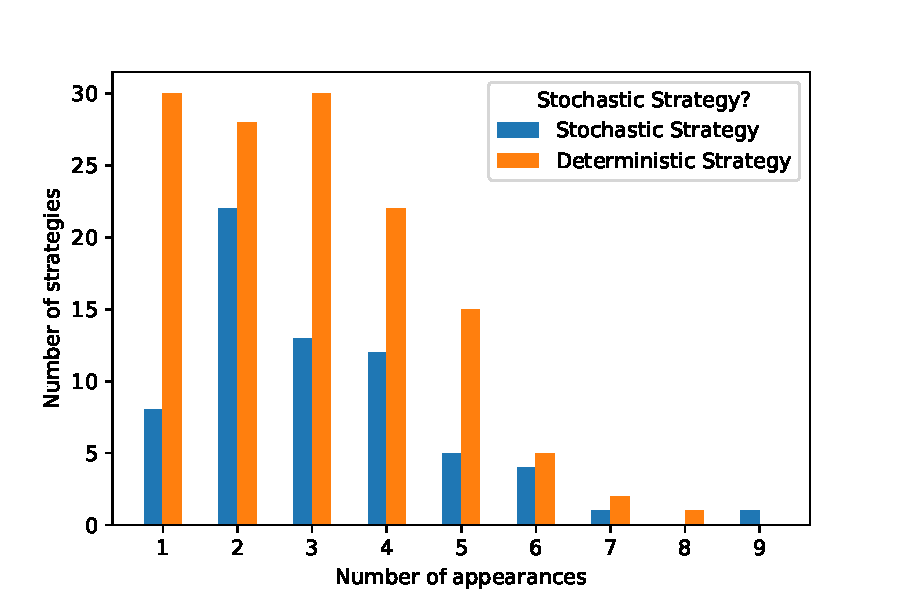
\includegraphics[width=\textwidth]{folk_thm/initial_analysis/strategy_appearances.pdf}
    \caption{A plot to show the ratio of stochastic to deterministic strategies randomly chosen throughout the experiment.}\label{fig:stochastic_chart}
\end{figure}

It is clear that there is a clear bias towards deterministic strategies
in this experiment. However, this is to be expected as running the following
code:
\begin{minted}{frame=lines, framesep=2mm, fontsize=\scriptsize, bgcolor=Cornsilk}{python}
    
    len(axl.filtered_strategies(filterset={"stochastic": True})), 
    len(axl.filtered_strategies(filterset={"stochastic": False}))

    (86, 156)
\end{minted}
it can be seen that over half the strategies coded into the Axelrod library are
classed as deterministic. Looking at Figure~\ref{fig:stochastic_chart} again,
observe, the majority of deterministic strategies were executed either once or
three times. On the other hand, a large proportion of the stochastic strategies
were played twice.

Further, the number of Nash equilibria obtained for each game was analysed and
their distributions with respect to the number of opponents of the
\textit{Defector} plotted. Executing the \textit{value_counts} method on the
`num_of_equilibria' column gave the conclusion that the majority of games
(131773) yielded one Nash equilibria with 28793 games obtaining 3 equilibria.
Also, the maximum number of equilibria yielded, 39, was for one game, which,
doing a search on the database, was found to be a six player game with
noise=0.1. The opponents of the \textit{Defector} were: \textit{Inverse
Punisher}; \textit{Prober}; \textit{PSO Gambler 2 _ 2 _ 2 Noise 05};
\textit{Handshake}; and \textit{More Tideman and Chieruzzi}.

Figure~\ref{fig:NE_violinplot} shows the distributions of the number of Nash
equilibria as per the number of players. As can be seen from the plot, the
variance in the number of equilibria increases with the number of players, apart
from when there were 6 players (5 opponents of the defector), where the spread
is maximum. This could be due to the 39 equilibria gained for one game as
discussed in the paragraph above. Looking now at the mean of the distributions,
observe that these are also slightly increasing as the number of players
increase. 

\begin{figure}      
    \centering
    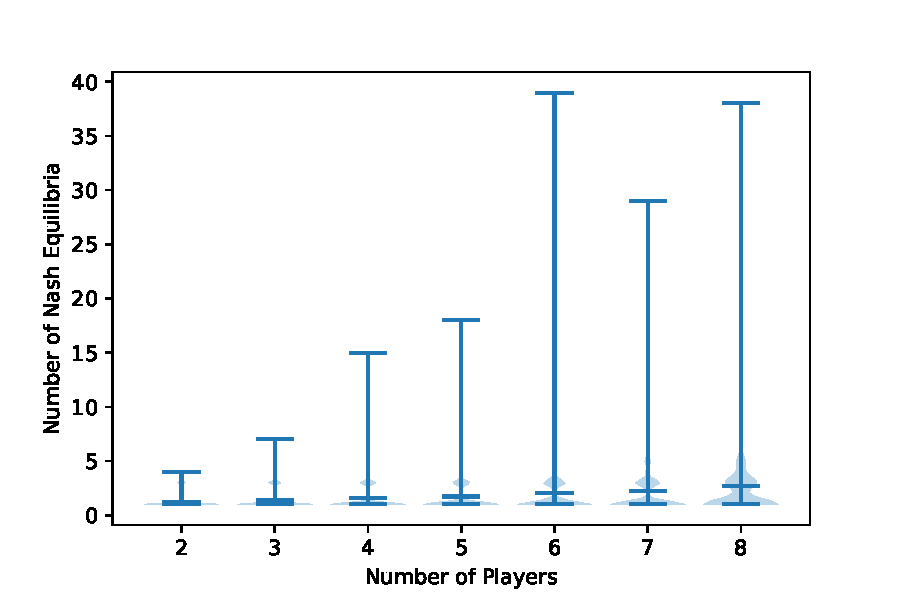
\includegraphics[width=\textwidth]{folk_thm/initial_analysis/player_num_of_equilibria_violinplot.pdf}
    \caption{A violinplot showing the distribution of the number of equilibria obtained for varying number of players.}\label{fig:NE_violinplot}
\end{figure}



\section{Analysis of the p-Threshold}\label{sec:Analysis_of_the_p-Threshold}
In order to analyse the \(p\)-thresholds of the tournaments, two csv files were
created containing the minimum, mean, median and maximum probabilities for each
set of tournaments. This was in order to gain as much information as possible
from tournaments which gave graphs as shown in Figure~\ref{fig:less_clear}. That
is, tournaments in which the number of repetitions was not sufficient to omit
the `noise' which can affect the results.

\begin{figure}
    \begin{subfigure}{.3\textwidth}
        \centering
        \includegraphics[width=\textwidth]{folk_thm/single_game/8/157/0.0/main.pdf}
        \caption{This was an eight player tournament with no added noise. The opponent strategies were: \textit{Tester}; \textit{Gradual Killer: (D, D, D, D, D, C, C)}; \textit{Win-Shift Lose-Stay: D}; \textit{Evolved FSM 16}; \textit{Limited Retaliate: 0.1, 20}; \textit{ZD-GEN-2: 0.125, 0.5, 3}; and \textit{Joss: 0.9}.}
    \end{subfigure}
    \begin{subfigure}{.3\textwidth}
        \centering
        \includegraphics[width=\textwidth]{folk_thm/single_game/5/80/0.0/main.pdf}
        \caption{This was a five player tournament with no added noise. The opponent strategies were: \textit{WmAdams}; \textit{Joss: 0.9}; \textit{Yamachi}; and \textit{Stochastic WSLS:\@ 0.05}.}
    \end{subfigure}
    \begin{subfigure}{.3\textwidth}
        \centering
        \includegraphics[width=\textwidth]{folk_thm/single_game/2/24/0.0/main.pdf}
        \caption{This was a two player tournament with no added noise. The \textit{Defector}'s opponent was \textit{Fortress3}.}
    \end{subfigure}
    \caption{Examples of plots where the \(p\)-threshold isn't as clear.}\label{fig:less_clear}
\end{figure}

The first csv file created ignored whether a game could be degenerate and, by a
small alteration, the second file contained only the non-degenerate games. This
was in order to help identify whether degeneracy has any effect on the
\(p\)-threshold. Within these files, other than the varying thresholds, the
information about the number of players, tournament strategy set and level of
noise was retained.

Firstly, an exploration into the overall \(p\)-thresholds is given.

\begin{figure}
    \begin{subfigure}{.45\textwidth}
        \centering
        \includegraphics[width=\textwidth]{folk_thm/main_analysis/min_p_thresh.pdf}
        \caption{A plot to show the minimum \(p\)-thresholds.}\label{subfig:min_p_thresh}
    \end{subfigure}
    \begin{subfigure}{.45\textwidth}
        \centering
        \includegraphics[width=\textwidth]{folk_thm/main_analysis/max_p_thresh.pdf}
        \caption{A plot to show the maximum \(p\)-thresholds.}\label{subfig:max_p_thresh}
    \end{subfigure}
    \caption{Plots to show the \(p\)-thresholds for all 1749 sets of tournaments.}\label{fig:min_max_p_thresh}
\end{figure}


\begin{figure}
    \begin{subfigure}{.45\textwidth}
        \centering
        \includegraphics[width=\textwidth]{folk_thm/main_analysis/mean_p_thresh.pdf}
        \caption{A plot to show the mean \(p\)-thresholds.}\label{subfig:mean_p_thresh}
    \end{subfigure}
    \begin{subfigure}{.45\textwidth}
        \centering
        \includegraphics[width=\textwidth]{folk_thm/main_analysis/median_p_thresh.pdf}
        \caption{A plot to show the median \(p\)-thresholds.}\label{subfig:median_p_thresh}
    \end{subfigure}
    \caption{Plots to show the \(p\)-thresholds for all 1749 sets of tournaments.}\label{fig:mean_median_p_thresh}
\end{figure}




\begin{figure}
    \begin{subfigure}{.45\textwidth}
        \centering
        \includegraphics[width=\textwidth]{folk_thm/main_analysis/non_degenerate_min_p_thresh.pdf}
        \caption{A plot to show the minimum \(p\)-thresholds.}\label{subfig:non_degen_min_p_thresh}
    \end{subfigure}
    \begin{subfigure}{.45\textwidth}
        \centering
        \includegraphics[width=\textwidth]{folk_thm/main_analysis/non_degenerate_max_p_thresh.pdf}
        \caption{A plot to show the maximum \(p\)-thresholds.}\label{subfig:non_degen_max_p_thresh}
    \end{subfigure}
    \caption{Plots to show the \(p\)-thresholds for all tournaments which led to non-degenerate games.}\label{fig:non_degen_min_max_p_thresh}
\end{figure}


\begin{figure}
    \begin{subfigure}{.45\textwidth}
        \centering
        \includegraphics[width=\textwidth]{folk_thm/main_analysis/non_degenerate_mean_p_thresh.pdf}
        \caption{A plot to show the mean \(p\)-thresholds.}\label{subfig:non_degen_mean_p_thresh}
    \end{subfigure}
    \begin{subfigure}{.45\textwidth}
        \centering
        \includegraphics[width=\textwidth]{folk_thm/main_analysis/non_degenerate_median_p_thresh.pdf}
        \caption{A plot to show the median \(p\)-thresholds.}\label{subfig:non_degen_median_p_thresh}
    \end{subfigure}
    \caption{Plots to show the \(p\)-thresholds for all tournaments which led to non-degenerate games.}\label{fig:non_degen_mean_median_p_thresh}
\end{figure}




\subsection{Effects of the Number of Players}\label{subsec:Effects_of_the_number_of_Players}


\begin{figure}
    \begin{subfigure}{.45\textwidth}
        \centering
        \includegraphics[width=\textwidth]{folk_thm/main_analysis/2player_mean_p_thresh.pdf}
        \caption{A plot to show the mean \(p\)-thresholds for all two player tournaments.}\label{subfig:2player_mean_p_thresh}
    \end{subfigure}
    \begin{subfigure}{.45\textwidth}
        \centering
        \includegraphics[width=\textwidth]{folk_thm/main_analysis/3player_mean_p_thresh.pdf}
        \caption{A plot to show the mean \(p\)-thresholds for all three player tournaments.}\label{subfig:3player_mean_p_thresh}
    \end{subfigure}
    

    \newline


    \begin{subfigure}{.3\textwidth}
        \centering
        \includegraphics[width=\textwidth]{folk_thm/main_analysis/4player_mean_p_thresh.pdf}
        \caption{A plot to show the mean \(p\)-thresholds for all four player tournaments.}\label{subfig:4player_mean_p_thresh}
    \end{subfigure}
    \begin{subfigure}{.3\textwidth}
        \centering
        \includegraphics[width=\textwidth]{folk_thm/main_analysis/5player_mean_p_thresh.pdf}
        \caption{A plot to show the mean \(p\)-thresholds for all five player tournaments.}\label{subfig:5player_mean_p_thresh}
    \end{subfigure}
    \begin{subfigure}{.3\textwidth}
        \centering
        \includegraphics[width=\textwidth]{folk_thm/main_analysis/6player_mean_p_thresh.pdf}
        \caption{A plot to show the mean \(p\)-thresholds for all six player tournaments.}\label{subfig:6player_mean_p_thresh}
    \end{subfigure}


    \newline


    \begin{subfigure}{.45\textwidth}
        \centering
        \includegraphics[width=\textwidth]{folk_thm/main_analysis/7player_mean_p_thresh.pdf}
        \caption{A plot to show the mean \(p\)-thresholds for all seven player tournaments.}\label{subfig:7player_mean_p_thresh}
    \end{subfigure}
    \begin{subfigure}{.45\textwidth}
        \centering
        \includegraphics[width=\textwidth]{folk_thm/main_analysis/8player_mean_p_thresh.pdf}
        \caption{A plot to show the mean \(p\)-thresholds for all eight player tournaments.}\label{subfig:8player_mean_p_thresh}
    \end{subfigure}
    \caption{Plots to show the mean \(p\)-threshold for varying numbers of opponents of the \textit{Defector}.}\label{fig:player_mean_p_thresh}
\end{figure}


\begin{figure}
    \centering
    \includegraphics[width=\textwidth]{folk_thm/main_analysis/player_mean_thresh_violinplot.pdf}
    \caption{A violinplot showing the distribution of mean \(p\)-thresholds for each number of opponents.}\label{fig:player_mean_thresh_violinplot}
\end{figure}


\subsection{Effects of Stochastic Players}\label{subsec:Effects_of_Stochastic_Players}






\subsection{Effects of Noise}\label{subsec:Effects_of_Noise}


\begin{figure}
    \begin{subfigure}{.45\textwidth}
        \centering
        \includegraphics[width=\textwidth]{folk_thm/main_analysis/0.0noise_mean_p_thresh.pdf}
        \caption{A plot to show the mean \(p\)-thresholds for all tournaments with no added noise.}\label{subfig:0.0noise_mean_p_thresh}
    \end{subfigure}
    \begin{subfigure}{.45\textwidth}
        \centering
        \includegraphics[width=\textwidth]{folk_thm/main_analysis/0.1noise_mean_p_thresh.pdf}
        \caption{A plot to show the mean \(p\)-thresholds for all tournaments with noise = 0.1.}\label{subfig:0.1noise_mean_p_thresh}
    \end{subfigure}
    

    \newline


    \begin{subfigure}{.3\textwidth}
        \centering
        \includegraphics[width=\textwidth]{folk_thm/main_analysis/0.2noise_mean_p_thresh.pdf}
        \caption{A plot to show the mean \(p\)-thresholds for all tournaments with noise = 0.2.}\label{subfig:0.2noise_mean_p_thresh}
    \end{subfigure}
    \begin{subfigure}{.3\textwidth}
        \centering
        \includegraphics[width=\textwidth]{folk_thm/main_analysis/0.3noise_mean_p_thresh.pdf}
        \caption{A plot to show the mean \(p\)-thresholds for all tournaments with noise = 0.3.}\label{subfig:0.3noise_mean_p_thresh}
    \end{subfigure}
    \begin{subfigure}{.3\textwidth}
        \centering
        \includegraphics[width=\textwidth]{folk_thm/main_analysis/0.4noise_mean_p_thresh.pdf}
        \caption{A plot to show the mean \(p\)-thresholds for all tournaments with noise = 0.4.}\label{subfig:0.4noise_mean_p_thresh}
    \end{subfigure}


    \newline


    \begin{subfigure}{.3\textwidth}
        \centering
        \includegraphics[width=\textwidth]{folk_thm/main_analysis/0.5noise_mean_p_thresh.pdf}
        \caption{A plot to show the mean \(p\)-thresholds for all tournaments with noise = 0.5.}\label{subfig:0.5noise_mean_p_thresh}
    \end{subfigure}
    \begin{subfigure}{.3\textwidth}
        \centering
        \includegraphics[width=\textwidth]{folk_thm/main_analysis/0.6noise_mean_p_thresh.pdf}
        \caption{A plot to show the mean \(p\)-thresholds for all tournaments with noise = 0.6.}\label{subfig:0.6noise_mean_p_thresh}
    \end{subfigure}
    \begin{subfigure}{.3\textwidth}
        \centering
        \includegraphics[width=\textwidth]{folk_thm/main_analysis/0.7noise_mean_p_thresh.pdf}
        \caption{A plot to show the mean \(p\)-thresholds for all tournaments with noise = 0.7.}\label{subfig:0.7noise_mean_p_thresh}
    \end{subfigure}
    \begin{subfigure}{.3\textwidth}
        \centering
        \includegraphics[width=\textwidth]{folk_thm/main_analysis/0.8noise_mean_p_thresh.pdf}
        \caption{A plot to show the mean \(p\)-thresholds for all tournaments with noise = 0.8.}\label{subfig:0.8noise_mean_p_thresh}
    \end{subfigure}
    \begin{subfigure}{.3\textwidth}
        \centering
        \includegraphics[width=\textwidth]{folk_thm/main_analysis/0.9noise_mean_p_thresh.pdf}
        \caption{A plot to show the mean \(p\)-thresholds for all tournaments with noise = 0.9.}\label{subfig:0.9noise_mean_p_thresh}
    \end{subfigure}
    \begin{subfigure}{.3\textwidth}
        \centering
        \includegraphics[width=\textwidth]{folk_thm/main_analysis/1.0noise_mean_p_thresh.pdf}
        \caption{A plot to show the mean \(p\)-thresholds for all tournaments with noise = 1.0.}\label{subfig:1.0noise_mean_p_thresh}
    \end{subfigure}
    \caption{Plots to show the mean \(p\)-threshold for varying levels of noise.}\label{fig:noise_mean_p_thresh}
\end{figure}

\begin{figure}
    \centering
    \includegraphics[width=\textwidth]{folk_thm/main_analysis/noise_mean_thresh_violinplot.pdf}
    \caption{A violinplot showing the distribution of mean \(p\)-thresholds for each level of noise.}\label{fig:noise_mean_thresh_violinplot}
\end{figure}



\subsection{Effects of Degeneracy}\label{subsec:Effects_of_Degeneracy}

\section{Multivariate Data Analysis}\label{sec:MV_Data_Analysis}

\section{Reliability of Data}\label{sec:Reliability_of_Data}

\subsection{Comparison of Databases}\label{subsec:Comparison_of_Databases}

\subsection{Accuracy of Thresholds}\label{subsec:Accuracy_of_Thresholds}